\documentclass{beamer}
\mode<presentation>
\usepackage{amsmath}
\usepackage{amssymb}
%\usepackage{advdate}
\usepackage{adjustbox}
\usepackage{subcaption}
\usepackage{enumitem}
\usepackage{multicol}
\usepackage{mathtools}
\usepackage{listings}
\usepackage{url}
\def\UrlBreaks{\do\/\do-}
\usetheme{metropolis}
%\usecolortheme{lily}
\setbeamertemplate{footline}
{
	\leavevmode%
	\hbox{%
		\begin{beamercolorbox}[wd=\paperwidth,ht=2.25ex,dp=1ex,right]{author in head/foot}%
			\insertframenumber{} / \inserttotalframenumber\hspace*{2ex} 
		\end{beamercolorbox}}%
		\vskip0pt%
	}
	\setbeamertemplate{navigation symbols}{}

	\providecommand{\nCr}[2]{\,^{#1}C_{#2}} % nCr
	\providecommand{\nPr}[2]{\,^{#1}P_{#2}} % nPr
	\providecommand{\mbf}{\mathbf}
	\providecommand{\pr}[1]{\ensuremath{\Pr\left(#1\right)}}
	\providecommand{\qfunc}[1]{\ensuremath{Q\left(#1\right)}}
	\providecommand{\sbrak}[1]{\ensuremath{{}\left[#1\right]}}
	\providecommand{\lsbrak}[1]{\ensuremath{{}\left[#1\right.}}
	\providecommand{\rsbrak}[1]{\ensuremath{{}\left.#1\right]}}
	\providecommand{\brak}[1]{\ensuremath{\left(#1\right)}}
	\providecommand{\lbrak}[1]{\ensuremath{\left(#1\right.}}
	\providecommand{\rbrak}[1]{\ensuremath{\left.#1\right)}}
	\providecommand{\cbrak}[1]{\ensuremath{\left\{#1\right\}}}
	\providecommand{\lcbrak}[1]{\ensuremath{\left\{#1\right.}}
	\providecommand{\rcbrak}[1]{\ensuremath{\left.#1\right\}}}
	\theoremstyle{remark}
	\newtheorem{rem}{Remark}
	\newcommand{\sgn}{\mathop{\mathrm{sgn}}}
	\providecommand{\abs}[1]{\left\vert#1\right\vert}
	\providecommand{\res}[1]{\Res\displaylimits_{#1}} 
	\providecommand{\norm}[1]{\lVert#1\rVert}
	\providecommand{\mtx}[1]{\mathbf{#1}}
	\providecommand{\mean}[1]{E\left[ #1 \right]}
	\providecommand{\fourier}{\overset{\mathcal{F}}{ \rightleftharpoons}}
	%\providecommand{\hilbert}{\overset{\mathcal{H}}{ \rightleftharpoons}}
	\providecommand{\system}{\overset{\mathcal{H}}{ \longleftrightarrow}}
	%\newcommand{\solution}[2]{\textbf{Solution:}{#1}}
	%\newcommand{\solution}{\noindent \textbf{Solution: }}
	\providecommand{\dec}[2]{\ensuremath{\overset{#1}{\underset{#2}{\gtrless}}}}
	\newcommand{\myvec}[1]{\ensuremath{\begin{pmatrix}#1\end{pmatrix}}}
		\let\vec\mathbf

		\lstset{
			%language=C,
			frame=single, 
			breaklines=true,
			columns=fullflexible
		}

		\numberwithin{equation}{section}

		\title{NCERT Presentation}
		\author{Arjun Pavanje,\\ EE24BTECH11005,\\IIT Hyderabad.\\}

		\date{\today} 
		\begin{document}

		\begin{frame}
			\titlepage
		\end{frame}

		\section*{Table of Contents}
		\begin{frame}
			\tableofcontents
		\end{frame}
		\section{Problem}
		\begin{frame}
			\frametitle{Problem Statement}
Of all the closed right circular cylindrical cans of given volume  $100 cm^3$, find the dimensions of the can which has minimum surface area \newline
    \end{frame}
		\section{Solution}
    \subsection{Solution}
    \begin{frame}
      \frametitle{Solution}
Surface Area of cylinder is given by, 
\begin{align}
  2\pi rh + 2\pi r^2
\end{align}
Volume of a cylinder is given by, 
\begin{align}
  \pi r^2 h
\end{align}
where $r$ is the radius of the cylinder, $h$ is the height of the cylinder.\newline
Given that volume is $100 cm^3$,
\begin{align}
  \pi r^2 h = 100\\
  h = \frac{100}{\pi r^2}
\end{align}
Equation $\brak{3.1}$ becomes,
\begin{align}
  \brak{\frac{200}{r} + 2\pi r^2}
\end{align}      

    \end{frame}
		\subsection{Theoretical Solution}
		\begin{frame}
      \frametitle{Theoretical Solution}
To minimize surface area, differentiate equation $\brak{1}$ and set it to zero,
\begin{align}
  \frac{4\pi r^3 - 200}{r^2}=0
\end{align}
value of $r$ at which satisfies is, $\brak{\frac{50}{\pi}}^{\frac{1}{3}}$. We can verify that this is a minima by differentiating equation $\brak{6}$,
\begin{align}
  \frac{400}{r^3} + 4\pi
\end{align}
Thus we see that at the above value of $r$, it is a minima.\newline
Can of given volume will have maximum surface area when radius is $\brak{\frac{50}{\pi}}^{\frac{1}{3}} cm$, height is $2\brak{\frac{\pi}{50}}^{\frac{1}{3}}$\newline
    \end{frame}
        \subsection{Computational Solution 1}
			\begin{frame}
      \frametitle{Computational solution 1}
      {\small
We need to minimize,
\begin{align}
  \brak{\frac{200}{r} + 2\pi r^2}
\end{align}
Applying gradient descent theorem,
\begin{align}
  r_{n+1} = r_n -\mu f^{\prime}\brak{r_n}
\end{align}
where $\mu$ is the step size,
\begin{align}
  f^{\prime}\brak{r_n} = -\frac{200}{r_n^2} +4\pi r_n
\end{align}
Final Difference Equation comes out to be, 
\begin{align}
  r_{n+1} = r_n\brak{1 - 4\pi} + \frac{200}{r_n^2} 
\end{align}
Taking inital guess as $2$, step size $0.01$, tolerence as $0.0001$.\newline
We get minimum value of $r$ to be $2.515397787094116 cm \approx \brak{\frac{50}{\pi}}^{\frac{1}{3}} cm$
      }
    \end{frame}
		
    \subsection{Computational Solution 2}
		\begin{frame}[fragile]
			\frametitle{Computational Solution 2}
We can also solve it using $cvxpy$ module in python. On running the code we get,\newline
Minimum value of $r$ is, $2.515299390016942 cm$, \newline Minimum surface area is, $ 119.26542080485049 cm^2$    
    \end{frame}
		\begin{frame}[fragile]
			\frametitle{Computational Solution}
			\begin{figure}[h!]
				\centering
				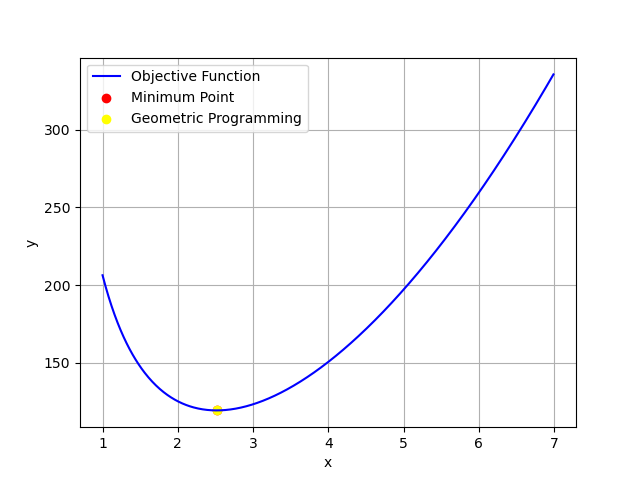
\includegraphics[width=1\columnwidth]{figs/fig.png}
				\label{stemplot}
			\end{figure}
	\end{frame}
	\end{document}
